%%%%%%%%%%%%%%%%%%%%%%%%%%%%%%%%%%%%%%%%%%%%%%%%%%%%%%%%%%%%%%%%%%%%%%%%%%%%%%%%
%2345678901234567890123456789012345678901234567890123456789012345678901234567890
%        1         2         3         4         5         6         7         8

\documentclass[letterpaper, 10 pt, conference]{ieeeconf}  % Comment this line out if you need a4paper
\usepackage{graphicx}

%\documentclass[a4paper, 10pt, conference]{ieeeconf}      % Use this line for a4 paper

\IEEEoverridecommandlockouts                              % This command is only needed if 
                                                          % you want to use the \thanks command

\overrideIEEEmargins                                      % Needed to meet printer requirements.

%In case you encounter the following error:
%Error 1010 The PDF file may be corrupt (unable to open PDF file) OR
%Error 1000 An error occurred while parsing a contents stream. Unable to analyze the PDF file.
%This is a known problem with pdfLaTeX conversion filter. The file cannot be opened with acrobat reader
%Please use one of the alternatives below to circumvent this error by uncommenting one or the other
%\pdfobjcompresslevel=0
%\pdfminorversion=4

% See the \addtolength command later in the file to balance the column lengths
% on the last page of the document

% The following packages can be found on http:\\www.ctan.org
%\usepackage{graphics} % for pdf, bitmapped graphics files
%\usepackage{epsfig} % for postscript graphics files
%\usepackage{mathptmx} % assumes new font selection scheme installed
%\usepackage{times} % assumes new font selection scheme installed
%\usepackage{amsmath} % assumes amsmath package installed
%\usepackage{amssymb}  % assumes amsmath package installed
\usepackage{mathtools}

\title{\LARGE \bf
CSE 598 Project Proposal: \\
Imitation Learning with Baxter Robot using Hi-Fives
}

\author{Michael Drolet, Frankie Liu, Evan Lam}


\begin{document}

\maketitle
\thispagestyle{empty}
\pagestyle{empty}


%%%%%%%%%%%%%%%%%%%%%%%%%%%%%%%%%%%%%%%%%%%%%%%%%%%%%%%%%%%%%%%%%%%%%%%%%%%%%%%%
\begin{abstract}
The goal of this project is to successfully learn hi-fives for human-robot interaction. We used an Imitation Learning approach by incorporating Bayesian Interaction Primitives \cite{c1}. Through expert-guided demonstrations, we train the robot to learn relationships between human and robot trajectories. We demonstrate that the robot is able to complete the interaction with a human and successfully issue a hi-five. We implemented the Bayesian Interaction Primitives to teach a Baxter Robot how to hi-five through imitation learning. Additionally, we compared the trajectories with human bio-mechanics data.
\end{abstract}


%%%%%%%%%%%%%%%%%%%%%%%%%%%%%%%%%%%%%%%%%%%%%%%%%%%%%%%%%%%%%%%%%%%%%%%%%%%%%%%%
\section{INTRODUCTION}
Teaching robots how to interact with humans is an interesting challenge in the field of Human Robot Interaction. The athletic and social components which make humans successful in daily interactions are often difficult to capture for robots. Nonetheless there are a variety of methods to teach robots to learn new tasks for human interaction. Imitation learning uses a human expert to guide the robot's interaction. Reinforcement Learning is another popular option for learning tasks that humans are experienced at. Bayesian Interaction approach is a probabilistic approach for teaching a robot.
\newline
\indent Our goal is to have a simple interaction that is able to be generalized across different robots using limited samples. The Bayesian Interaction approach enables a simple interaction which can be generalized using limited samples. On the other hand, using a Reinforcement Learning approach would require a significant number of demonstrations in order for the robot to learn the hi-five interaction.
\newline
\indent For our project, we train a Baxter robot which is traditionally an industrial robot built by Rethink Robotics. This Baxter robot is refitted in a friendly bear costume. We hope that by developing interactions for this Baxter robot, we can create an emotional support robot which can provide people comfort in times of emotional distress.
\newline
\begin{figure}[h]
\centering
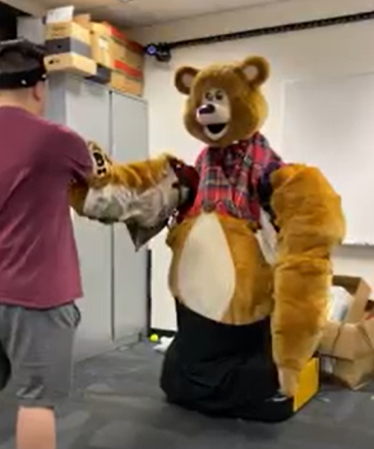
\includegraphics[width=0.18\textwidth]{Bear.PNG}
\caption{Example of human hi-fiving Baxter}
\end{figure}

\section{Related Work}

\subsection{Bayesian Interaction Primitives}
The Bayesian Interaction Primitive (BIP) framework is a novel and powerful approach that is being used by the Interactive Robotics Lab at Arizona State University. This SLAM inspired algorithm is useful for encoding spatiotemporal information about the interaction into a state space. BIP approximates each dimension using a weighted linear combination of time-dependent basis functions. In this case, we are using Gaussian basis functions. Included in a state vector are the weights for every basis function, the phase, and phase velocity. As a result, BIP allows us to infer the current state, given previous states (demonstrations) and current observations. Formatting this probabilistically allows the inference to be done using Bayes Filters (in particular, a Kalman Filter) during testing to guide the robot. Since the robot's degrees of freedom are no longer being observed during testing, the BIP framework is based on obtaining a partial observation of the current state to generate the positions/variables of the whole state space. This approach is effective for learning on different types of robots, as there is no domain specific knowledge encoded into the algorithm.

\section{Problem Statement}
The goal of this project is for the Baxter robot to successfully issue hi-fives. Our design consideration consists of a quick hi-five with a high success rate. We did most of our training and demonstrations on the Baxter robot, we also integrate our work with the VREP simulation tool.

\subsection{Teaching Baxter}

We trained two different primitives: a slow hi-five and a faster (more realistic) hi-five for our experiments. The Intrpim library was used to generate a model for our different primitives. We then evaluated the performance of each primitive and tested the models. The first model, which had more training examples, did much better than the second model. One of the issues encountered with the second model was that the rosbags were too long, so there was too much noise (only the first half was relevant). After trimming the bags to the correct length, we got worse performance. This leads us to believe that the bags were incorrectly trimmed, or something erreneous happened along the way. However, trimming the first set bags to the correct length improved the performance greatly. With that being said, our first interaction was a success. Due to the current cirumstances, we weren't able to verify whether the second interaction can be improved, as we need the physical robot to collect new training samples.

We used the Extended Kalman Filter (EKF) to perform the filtering in the experiment, as this filter is suitable for smaller sample sizes (compared to the Extended Kalman Filter) and offers good performance in practice.

\subsection{Data Generation}
We collected subject data by using the Optitrack motion capture system, where 3D poses were collected at 120 Hz. Subjects wore a headband and two gloves that are equipped with motion capture markers. By using only three degrees of freedom, we avoid performing inference in a space that is too high-dimensional. After all, hands and head position are likely the only relevant information needed to perform a successful hi-five. We used ROS as our communication protocol and to handle messages.

\begin{figure}[h]
\centering
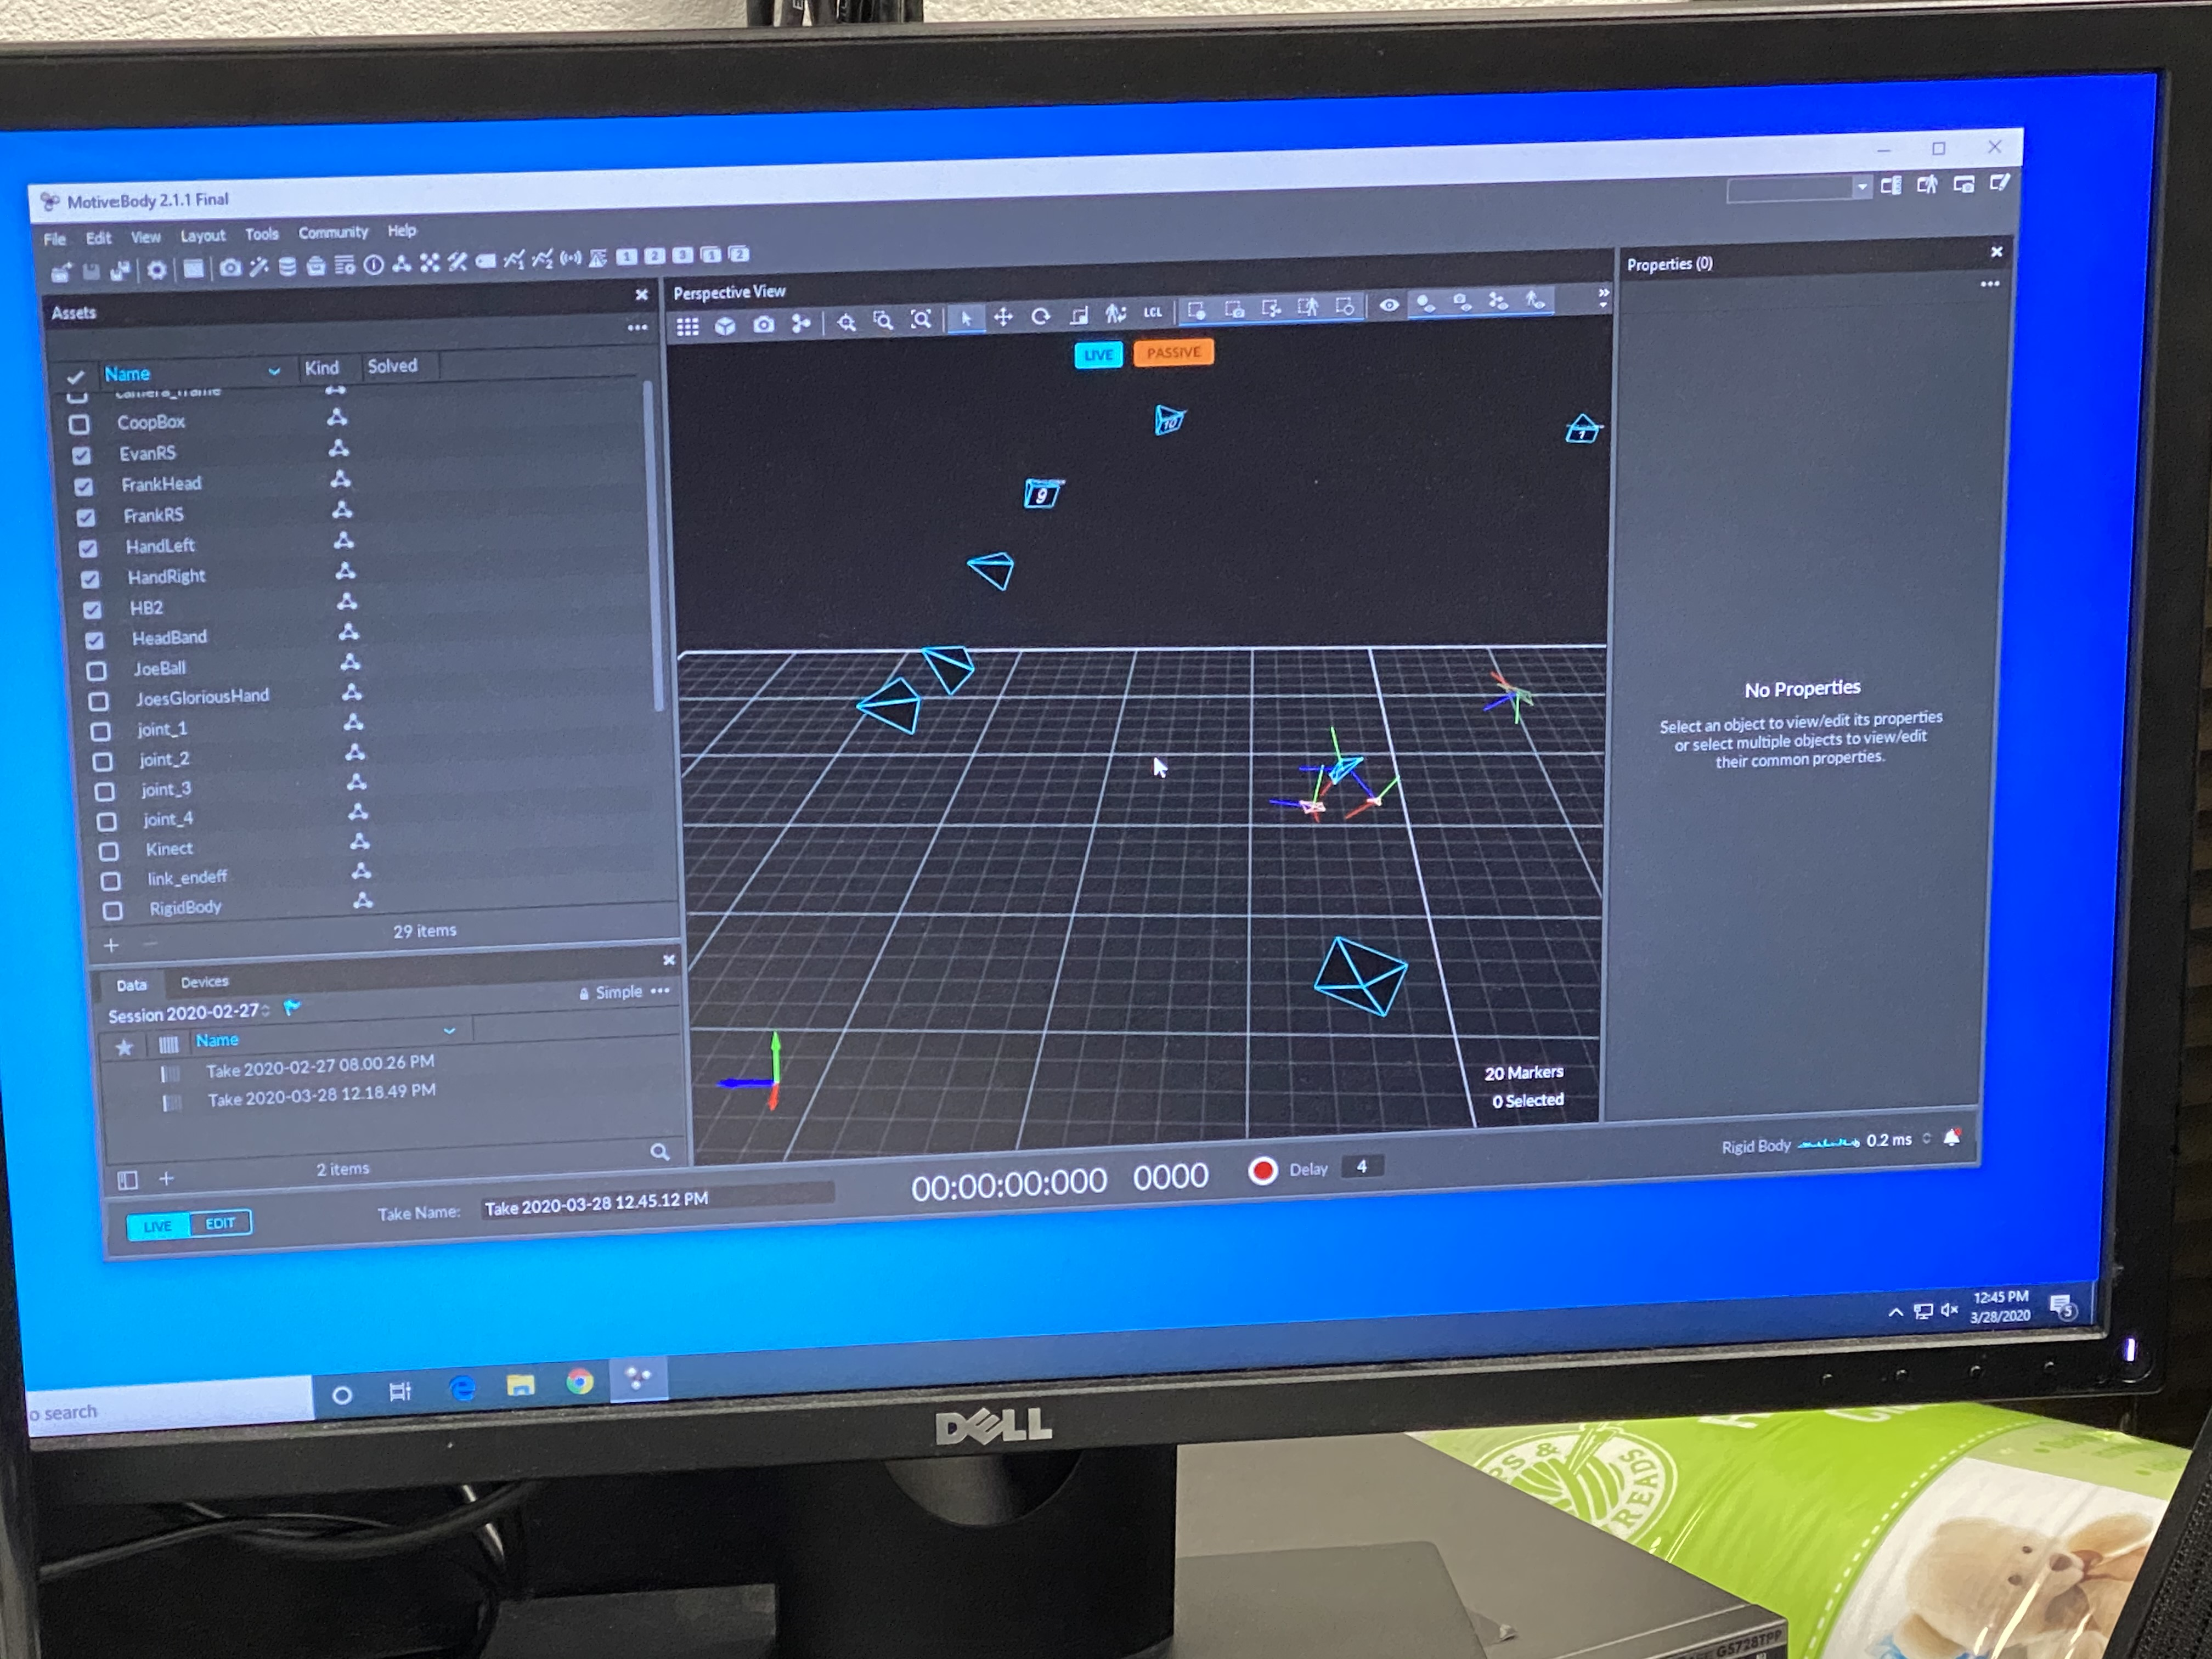
\includegraphics[width=0.5\textwidth]{Optitracker.jpg}
\caption{Optitracker application running}
\end{figure}

\subsection{Implementation}
A huge advantage of using the in-person Baxter robot is that we are able to find joint angle key frames for the training pose easily. For example, we put the robot into puppet mode and then recorded its key positions for a hi-five. Then, all that is required is to interpolate between these points to obtain a motion sequence. This method allowed us to quickly create different hi-five poses and allows us to come up with new poses if we decide to improve our hi-five motion. Lastly, the biggest benefit of using the Baxter in-person is that we have access to a controlled environment- with an Optitrack system, high speed network, and device drivers all configured- so that development and deployment is seamless.
\newline
\indent In order to train the Baxter robot, our group conducted approximately 75 in-person demonstrations (hi-fives) on the Baxter robot. Most of these test hi-fives were done using Frankie as the HRI partner, however we did not want our model to overfit the trajectories by using only one person. Therefore, we decided to also use Evan as a HRI partner during training. The hi-five was generated using key frames. We trained the Baxter robot on two different hi-five interaction types. Our first hi-five was very segmented and tried to mimic a robot movement. Our second hi-five was more fluid and smooth like a natural hi-five between two people. 

\subsection{Interaction Analysis and Bio-mechanic Analysis}

To complete a bio-mechanical analysis, we first captured a hi-five between two actual humans to get a sense of the motion. Optitrack sensors were placed on the participants' heads, right elbows, and right wrists. The three graphs in Fig. 3 show the x,y, and z positions of the both participants' right wrist. 
\begin{figure}[h]
\centering
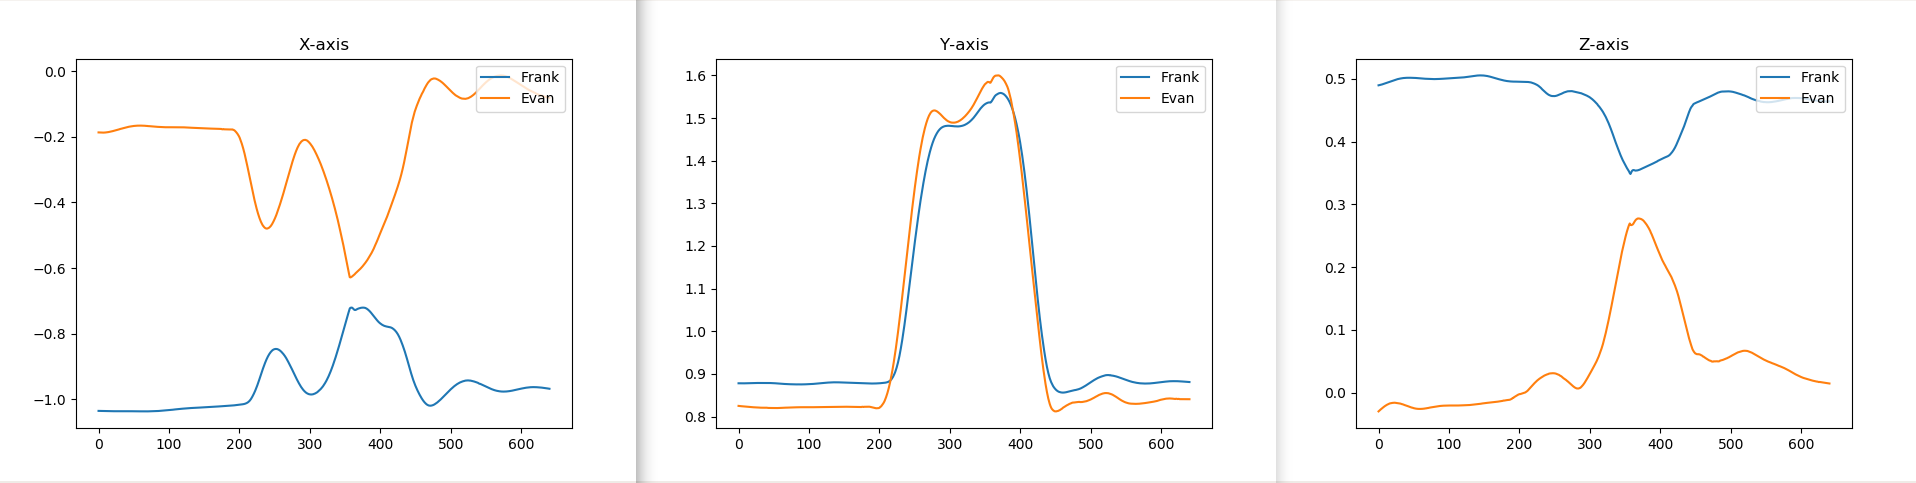
\includegraphics[width=0.5\textwidth]{biomechanics.png}
\caption{Human-human hi-five}
\end{figure} 
\newline
\indent From the graphs, we can see that the y-axis in this case likely represents the vertical axis, as the position of both participants wrists within the y-axis are almost the same throughout the entire duration of the hi-five. In a natural hi-five between two people, the participants both move their hands across their body to meet at a center point, resulting in the significant movement in the x-axis and z-axis, towards a single position, seen in the graphs in Fig. 3.
\newline
\indent Next, we analyzed the data captured from a hi-five between a person and the robot using the initial hi-five model that we developed. Optitrack sensors were placed on the participant's head, right wrist, and left wrist. Data for the Baxter robot was collected directly from it using the respective ROS topics. The three graphs in Fig. 4 show the x,y and z positions of the human's right wrist, and the robots, right "hand".
\begin{figure}[h]
\centering
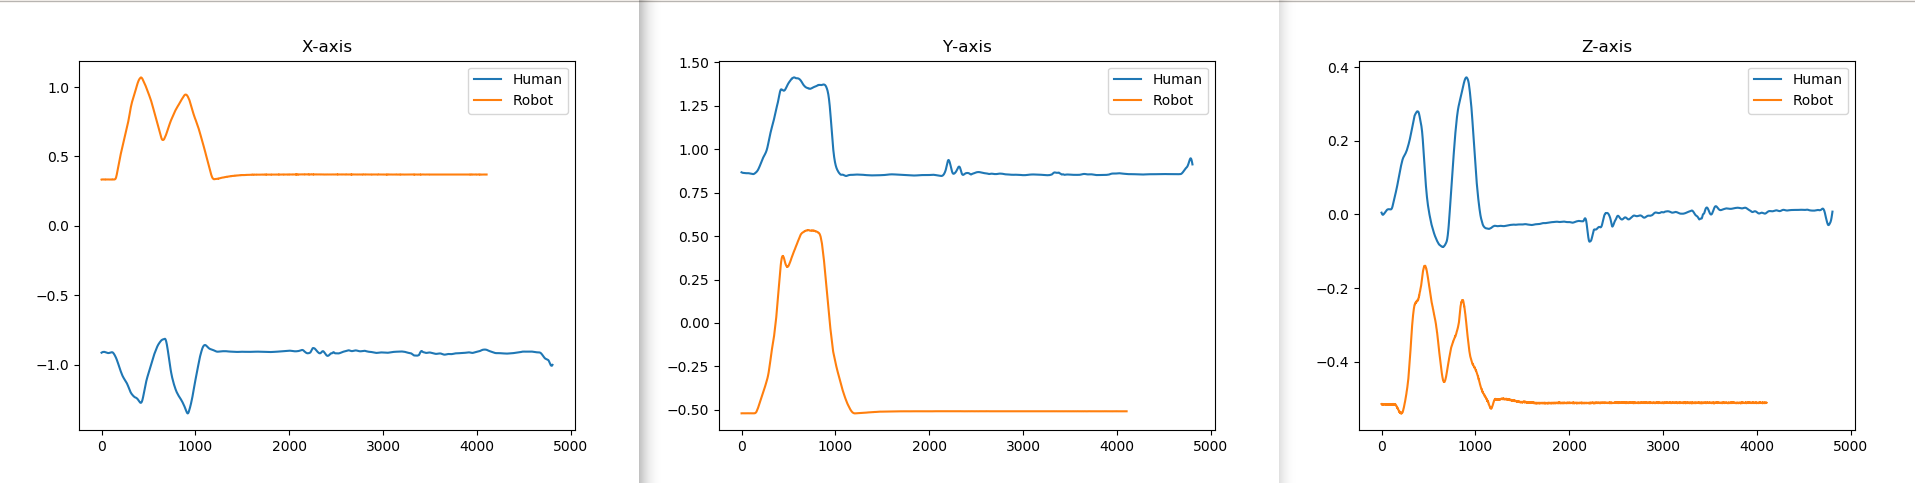
\includegraphics[width=0.5\textwidth]{oldfive.png}
\caption{Old human-robot hi-five. Note: data after about 1250 on time axis is extraneous}
\end{figure}
\newline
\indent The first thing to note here is that the data for the human is reported by the Optitrac system while the data for the robot is reported by the Baxter itself. This results in the points being mapped with respect to different origins, as shown in the y-axis graph, which once again represents the vertical axis, since the max height of the human's wrist is show to be significantly higher than the max height of the robot's "hand" despite the fact that they are at the same physical height at the time of the hi-five (around 800 on the time axis). This also causes the x-axis and y-axis graphs to look significantly different from the graphs generated from the human-human hi-five. 
\newline
\indent The overall movement patterns of each participant of the human-robot hi-five largely match the movement patterns of each participant of the human-human hi-five, even if the positions do not necessarily match up do to the different origin points as previously explained. While the overall patterns do match, the movement is much more jagged due to the stiff nature of the first hi-five model that we created.
\newline
\indent Finally, we analyzed the data captured from a hi-five between a person and the Baxter robot using the revised hi-five model that we developed. The same setup was used as the data collected from the original human-robot hi-five. The three graphs in Fig. 5 show the x,y and z positions of the human's right wrist, and the robots, right "hand".
\begin{figure}[h]
\centering
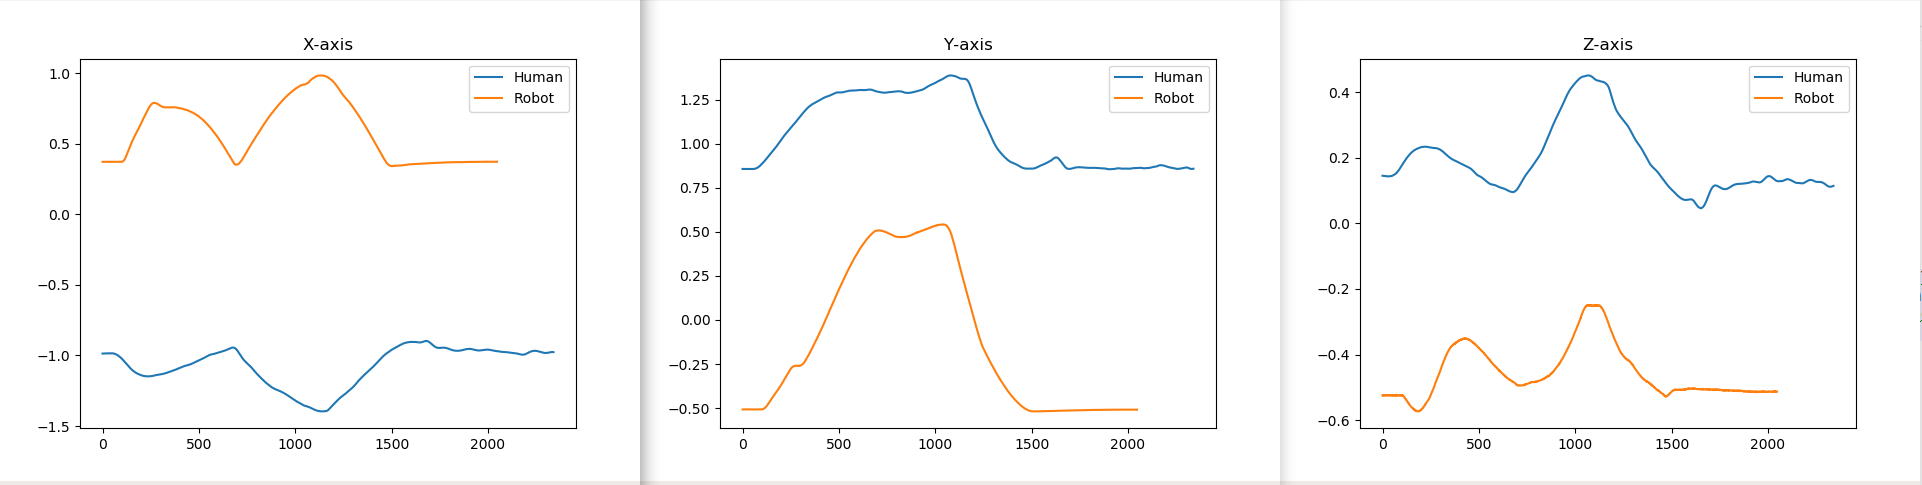
\includegraphics[width=0.5\textwidth]{newfive.png}
\caption{New human-robot hi-five}
\end{figure}
\newline
\indent Once again, the origin points used by the Optitrac system and the Baxter robot are different, resulting in the graphs looking significantly different from the human-human hi-five graphs. However, the overall movement patterns of each participant for the new human-robot hi-five match the movements of the participants in the human-human hi-five. With the new hi-five model, we also noticed that the movement within each axis was much more smooth compared to the movements from the old hi-five model, indicating our new model completes the hi-five in a more natural way that better mimics an actual human hi-five.
\newline
\indent To get a better comparison between the new robot hi-five model and an actual hi-five between two humans, we computed the correlation coefficients comparing the robot from the human-robot hi-five (new model) to the first human participant in the human-human hi-five:
\[
corrcoef(x)_{robot, human_1} = \begin{bmatrix}
	1 & -0.45045106 \\
	-0.45045106 & 1
\end{bmatrix}
\]
\newline
\[
corrcoef(y)_{robot, human_1} = \begin{bmatrix}
	1 & 0.53274616 \\
	0.53274616 & 1
\end{bmatrix}
\]
\newline
\[
corrcoef(z)_{robot, human_1} = \begin{bmatrix}
	1 & 0.25234082 \\
	0.25234082 & 1
\end{bmatrix}
\]
\newline
We also computed the correlation coefficients comparing the human from the human-robot hi-five (new model) to the second human participant in the human-human hi-five:
\[
corrcoef(x)_{human, human_2} = \begin{bmatrix}
1 & -0.31119984 \\
-0.31119984 & 1
\end{bmatrix}
\]
\newline
\[
corrcoef(y)_{human, human_2} = \begin{bmatrix}
1 & 0.56795077 \\
0.56795077 & 1
\end{bmatrix}
\]
\newline
\[
corrcoef(z)_{human, human_2} = \begin{bmatrix}
1 & -0.55262954 \\
-0.55262954 & 1
\end{bmatrix}
\]
\newline
From the above correlation coefficient matrices we see that the corresponding co-variance values from each axis in the robot to human1 comparison matrices is fairly similar to the co-variance values from each axis in the human to human2 comparison matrices. This indicates to us that our interaction with the robot is similar to the interactions between the humans. Therefore, the second hi-five model that we designed is good at matching a natural hi-five between two humans.

\subsection{Simulation Integration} 
The simulation tool we are using is VREP. This is a nice tool since its interface is user-friendly and there are useful resources to begin developing with it. We were considering using Gazebo due to its ability to integrate tightly with ROS. However, Gazebo appeared to be heavy compared to other simulators. We ultimately decided on VREP. 
\newline
\indent
One of the challenges we faced while using VREP was that its interface is different than the way we currently interact with the Baxter robot. The simulator has commands to set joint angles, joint velocities, and other options by using the built-in commands. However, we are using ROS topics within the IntPrim framework to control the Baxter robot. Consequently, switching from simulation to real-life would require a large number of code changes and a need to maintain two different types of controllers. 
\newline
\indent A work-around lead us to looking into using ROS topics for the VREP simulator, and using PyRep to handle the callbacks from receiving a message. PyRep can call internal LuaScript functions in the simulator, and has greater speed than the Blue Origin (simx). This means that the high frequency topics would be handled better using this PyRep/ROS integration, compared to vanilla VREP, and also gives us the ability to only maintain one ROS controller for both the simulation and real Baxter robot. The next challenge is to figure out which components should be done in-person (which is difficult due to the virus), and see which components can be done by using the simulator. 


\section{Current Limitations and Future Work}
Some of the parameters that need to be tuned are the number of basis functions per degree of freedom and the scaling factor for each. This is done through a grid-search that tests various combinations during testing and reports the configuration that results in the lowest Mean Absolute Error (MAE) from the ideal trajectory.

\section{Conclusion}
In the future, we plan to finish writing the ROS subscribers and PyRep interfaces in VREP. This will allow us to do offline experiments (simulations, per say) and when/if things subside with the virus, we can test the results in person. Additionally, we plan to meet and use the Optitrack system for the biomechanical analysis, as this will provide us with the most accurate results.

\addtolength{\textheight}{-12cm}   % This command serves to balance the column lengths
                                  % on the last page of the document manually. It shortens
                                  % the textheight of the last page by a suitable amount.
                                  % This command does not take effect until the next page
                                  % so it should come on the page before the last. Make
                                  % sure that you do not shorten the textheight too much.

%%%%%%%%%%%%%%%%%%%%%%%%%%%%%%%%%%%%%%%%%%%%%%%%%%%%%%%%%%%%%%%%%%%%%%%%%%%%%%%%



%%%%%%%%%%%%%%%%%%%%%%%%%%%%%%%%%%%%%%%%%%%%%%%%%%%%%%%%%%%%%%%%%%%%%%%%%%%%%%%%



%%%%%%%%%%%%%%%%%%%%%%%%%%%%%%%%%%%%%%%%%%%%%%%%%%%%%%%%%%%%%%%%%%%%%%%%%%%%%%%%

\begin{thebibliography}{99}
\bibitem{c1} J. Campbell, A. Hitzmann, S. Stepputtis, S. Ikemoto, K. Hosoda, and H. Ben Amor. Learning Interactive Behaviors for Musculoskeletal Robots Using Bayesian Interaction Primitives. IEEE/RSJ International Conference on Intelligent Robots and Systems (IROS), Macau, China, November 2019.
\end{thebibliography}




\end{document}
